	\documentclass[14pt]{extreport}
\usepackage{extsizes}
	\usepackage[frenchb]{babel}
	\usepackage[utf8]{inputenc}  
	\usepackage[T1]{fontenc}
	\usepackage{amssymb}
	\usepackage[mathscr]{euscript}
	\usepackage{stmaryrd}
	\usepackage{amsmath}
	\usepackage{tikz}
	\usepackage[all,cmtip]{xy}
	\usepackage{amsthm}
	\usepackage{varioref}
	\usepackage[ margin=1in]{geometry}
	\geometry{a4paper}
	\usepackage{lmodern}
	\usepackage{hyperref}
	\usepackage{array}
	\usepackage{float}
	\usepackage{easytable}
	 \usepackage{fancyhdr}\usepackage{longtable}
	 \usetikzlibrary{shapes.misc}
	 \newcommand\ang[1]{$#1{}^o$}
\newlength{\taillecellule}
\setlength{\taillecellule}{2cm}
\newcolumntype{C}{@{}>{\centering\arraybackslash}p{\taillecellule}@{}}

\renewcommand{\theenumi}{\alph{enumi})}
\usepackage{pstricks,multido}
\usepackage{arrayjob}
\usepackage{calc,xlop}
\tikzset{cross/.style={cross out, draw=black, minimum size=2*(#1-\pgflinewidth), inner sep=0pt, outer sep=0pt},
%default radius will be 1pt. 
cross/.default={1pt}}

	\pagestyle{fancy}
	\theoremstyle{plain}
	\fancyfoot[C]{\empty} 
	\fancyhead[L]{Devoir maison}
	\fancyhead[R]{13 mai 2024}
	
	
	
	\title{Devoir maison}
	\date{}
	\begin{document}



\subsection*{Exercice 1 : Calculs}  % 4 points


Posez et effectuez les calculs suivants : 
\begin{enumerate}
\item $341,45 + 24, 901 = $
\item $341,45 - 24, 901 =  $
\item $43$ h $46$ min + $4$h $55$ min = 
\item $43$ h $46$ min - $4$h $55$ min = 
\item $96,2 + 43, 865 + 514,019 = $
\item $200,101 - 10, 013 =  $
\item $52 \times 83,12 = $
\item $ 3,18 \times 529,85 = $
\end{enumerate}


\subsection*{Exercice 2 : Figure}

On considère les deux figures suivantes : 

\begin{figure}[H]
\center 
\begin{tikzpicture}[scale =1.3]
\draw (-2, 0) -- (2, 0) arc (0: 180 :2);
\draw (-2, 0) -- (2, 0) arc (0: 180 :2);
\draw[<->] (-2, -.2) -- (2, -.2); 
\draw (0, -.5) node {$7 \ cm$};
\draw[white](0,-1)--(3,-1);
\end{tikzpicture}
\begin{tikzpicture}[scale =1.3]
\draw[dotted](-2, 0) -- (2, 0);
\draw(2,0) arc (0: 180 :2) arc (180:360: 1) arc(180:0:1);
\draw(2,0) arc (0: 180 :2) arc (180:360: 1) arc(180:0:1);
\draw[<->] (2, -.2) -- (0, -.2); 
\draw (1, -.5) node {$4 \ cm$};
\end{tikzpicture}
\end{figure} 
\begin{enumerate}
\item Calculer une valeur exacte du périmètre de la première figure. Donnez ensuite une valeur approchée au millimètre. 

\item Calculer une valeur exacte du périmètre de la seconde figure. Donnez ensuite une valeur approchée au millimètre. 

\item Calculer une valeur exacte de l'aire de la première figure. Donnez ensuite une valeur approchée au millimètre carré. 

\item Calculer une valeur exacte de l'aire de la seconde figure. Donnez ensuite une valeur approchée au millimètre carré. 

\end{enumerate}  

\subsection*{Exercice 3 - Théorème de Pythagore sur un exemple}

On considère la figure suivante, constituée de quatre triangles rectangles identiques à l'intérieur d'un carré. On considère que le côté de carreau mesure $1$ centimètre

$$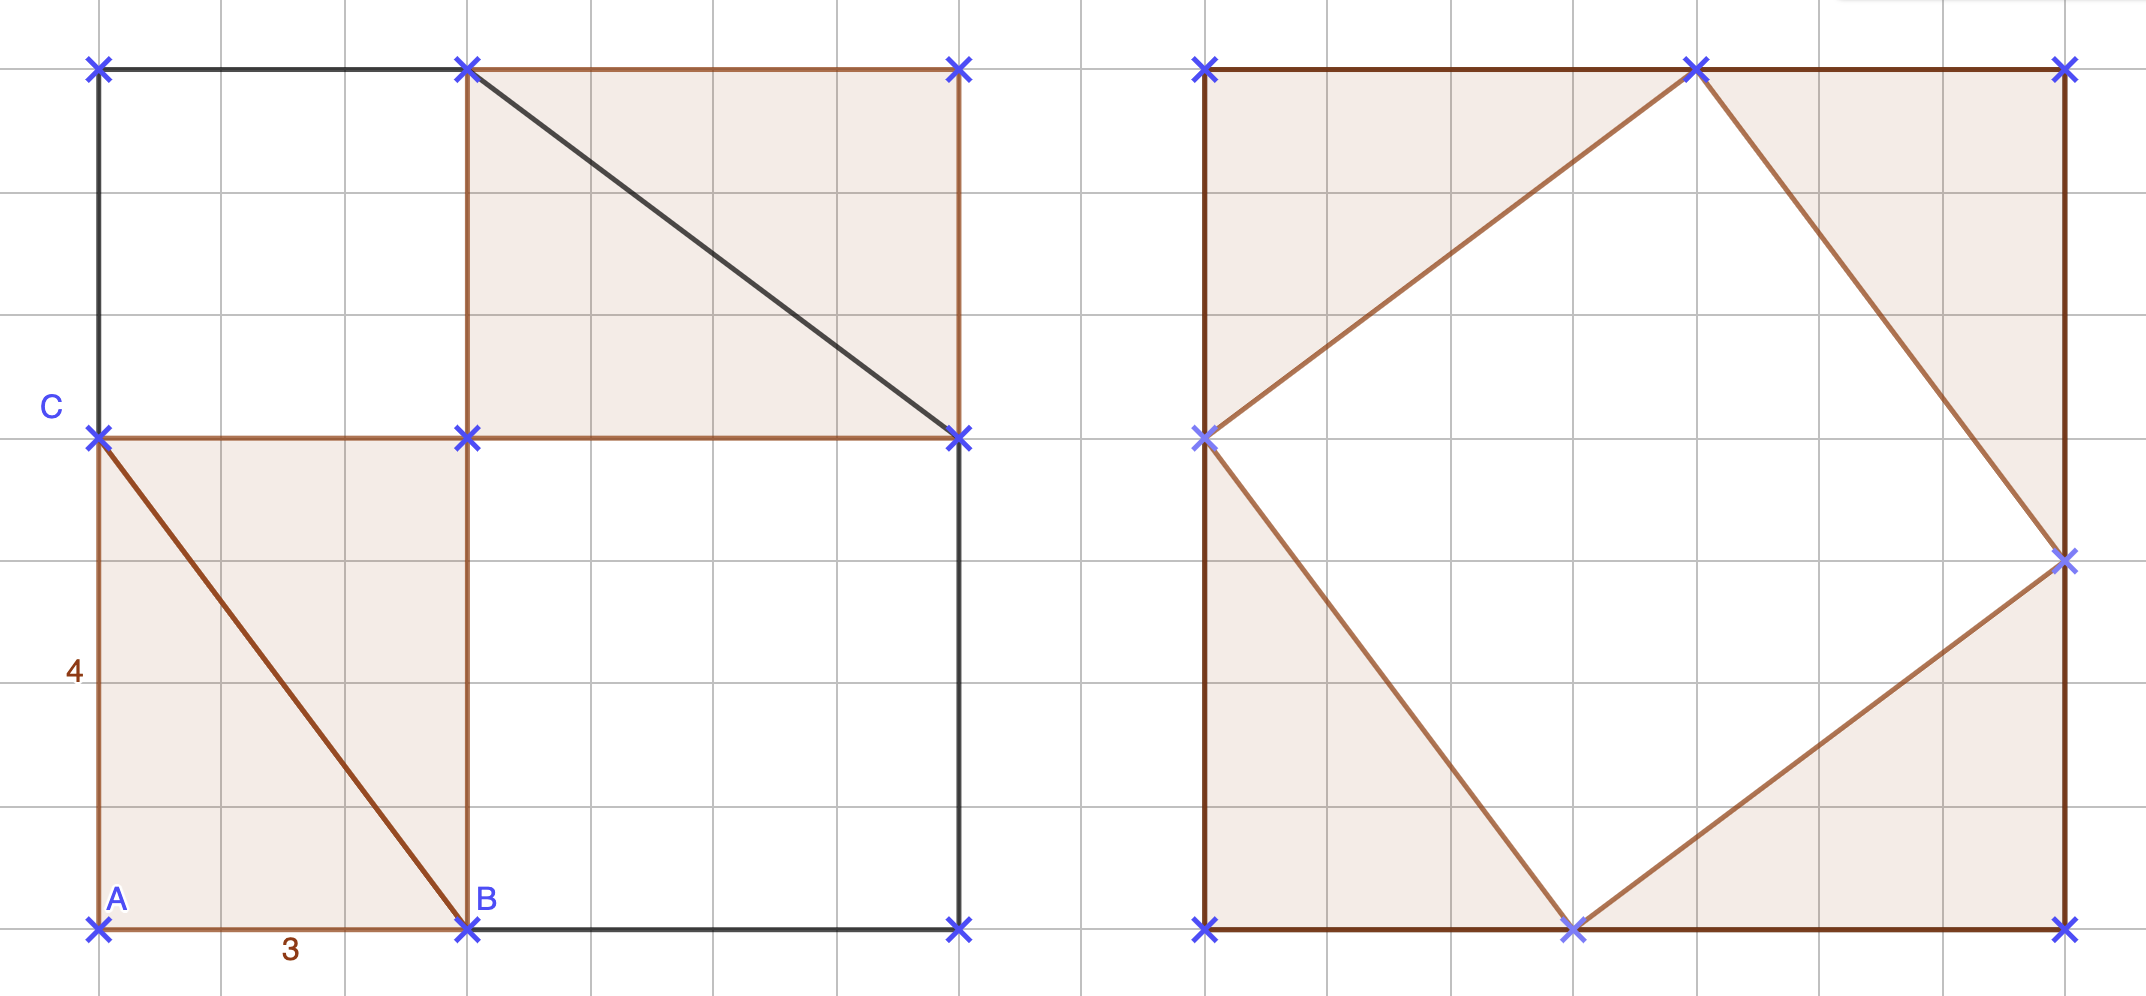
\includegraphics[width = 18cm]{Pythagore}$$
 \begin{enumerate}
 \item Montrer que la zone non coloriée de la figure de gauche mesure $25$ cm${}^2$. 
 \item Justifier que les figures de gauche et de droite ont la même surface non coloriée. 
 \item Quel est donc la longueur du côté du trou carré de la figure de droite ? 
 \item Conclure que $BC\times BC = AB\times AB + AC\times AC$. 
 \end{enumerate}
 
\end{document}